\cleardoublepage
\singlespacing
\chapter{SYSTEM DESIGN}
\label{c:design}
\doublespacing\nointerlineskip

\begin{comment}
Niels:about the tradeoffs in determining the deployment from your fault
tolerance perspective
Penn:Remember what the prof told me, about policy, first fit, last fit, etc
\end{comment}

%This chapter discussed the tradeoffs in determining optimal deployment for fault tolerance system such as RASCO. First it gives an overview of why it is a problem that we need to reconfigure the underlying network in a larger scale and how it is a problem to the system in itself in the long run. Then we will describe the deployment problem in the next section. Lastly, we identify certain tradeoffs in deployments for fault tolerance that could influence the system in a big way.

\section{System Design}
\label{s:sd}

The design for fault tolerance for WuKong is guided by the goals of WuKong to
have extensibility and flexibility. 

We want to support user policy that could configure how much nodes
should provide redundancy for a component to ensure certain level of
availability, and we want to be able to support for every component in the
application.  We also want the heartbeat protocol to reach the entire network in
an efficient way, the distribution of WuObjects in the network are not always be
ideal and evenly spread out in the network, thus heartbeat protocol designed
around strips will not be able to cover the whole network or to be optimized, so
by removing strip ordering from the concerns of heartbeat protocol design,
heartbeat protocol could be more efficient and adapatble.

\subsection{Fault Tolerance Policy for WuKong}

% No cowboy surprises here
\begin{comment}
\subsection{User Policy Framework}

\begin{figure}[h!]
\caption{A user component policy dialog}
\centering
    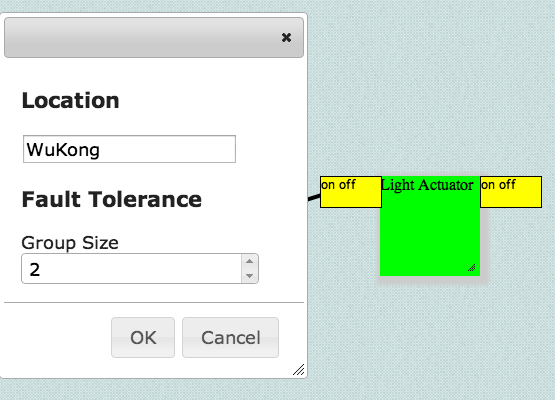
\includegraphics[width=\linewidth]{figures/fbp-policy}
\label{fig:fbp-policy}
\end{figure}

Many M2M applications are heavily influenced by user preferences and current
environmental context, as users and objects are mobile and application
requirements and policy could change in time. Users are able to specify
user policy for every component in the FBP and the application as a whole as
illustrated in Figure~\ref{fig:fbp-policy}

\subsubsection{Fault Tolerance policy}

M2M applications are inherently distributed, and hence it is inherently prone
to failures since all nodes are running autonomously unattended for a long
period of time where the external enviornmental influences could break and shut
down the devices easily. Fault Tolerance policy enables users to specify
relevent policy for tolerating failures in the granular level.
\end{comment}

\begin{comment}
Niels suggested that I show that I am aware of such issue with determining
optimality for deployment which is not clear for WuKong yet, there are many
ways or metrics to optimize for, all I can do in this work is to identify some
tradeoffs certain deployment for fault tolerance could influence the system
with certain metrics.

Limits will be hard to define here
\end{comment}

%RASCO achieves this by introducing the use of strips. Strips
%enable the system to track, maintain replicas and maintain consistency in the
%presence of failures. However, the number of failures RASCO can handle is still
%limited by the number of spare nodes that could provide required services. It is
%possible after a large change in the network, none of the nodes providing
%a service is there anymore, so it is impossible for the newly joined
%nodes to tap in and take over. To handle this large and permanent changes,
%WuKong supports a system progression framework that could handle such large
%change in the underlying network with dynamic \emph{reconfiguration}. WuKong
%reconfiguration reassigns associations between software components and hosts.
%But it does not have a solution to what the new assignment would look like.
%This deployment problem is a gap that should be considered.

%In the case of RASCO where deployment has to be continuously adjusted, the
%deployment problem is more of a online problem, so there is a tighter limit on
%time available to compute the assignment and strips, which makes the problem 
%a lot more interesting.

\section{Optimal deployment}

The problem of deploying a specific distributed system onto a network structure
typically consists of mapping the components of the system onto the hosts of
the network. The mapping is subject to constraints. In the case for RASCO, the
constraints are whether a node supports certain service to host certain
components, and how much communication overhead would induce from the
assignment to maintain consistency for the strips, and from the perspective of
WuKong, some components need to seaparate from other components to achieve
fault tolerance, and some needs to place together to function properly.

Determining such an optimal deployment is a \emph{combinatorial optimization}
problem. Combinatorial optimization problems are generally extremely
challenging computationally. However, the problem is ubiquitous as it happens
all around our lifes, whether it is companies trying to assign limited
resources to meet certain objectives, or institutions allocating resources to
its staff members to minimize cost, are examples of combinatorial optimization
problems. However it is difficult to predict what will and what will not work.
It is unlikely that a single approach will be effective on all problems or 
instances of the same problems. As we also want the system to come up with a solution within a time limit, there is a time constriant on the algorithms. So finding a good balance between the \emph{quality} of a solution of the \emph{time} it takes to come up with a good enough solution is critical.




\subsection{Reconfigurable Redundancy Architecture for Service-Oriented WSNs}

To keep track of heterogeneity of resources in distributed networks, WuKong
proposed WuClasses and WuObjects, as part of profile framework, to model after
physical resources such as sensor, actuators and virtual resources such as
computation, arithmatic.~\cite{Reijers} Each device host one or many WuObjects
where each represents the gateway to a certain hardware or virtual resource of
which the host could provide as a service.

\subsection{Strip}
\label{s:ss}

\begin{figure}[h!]
\caption{An example network with several strips}
\label{fig:strip1}
\centering
    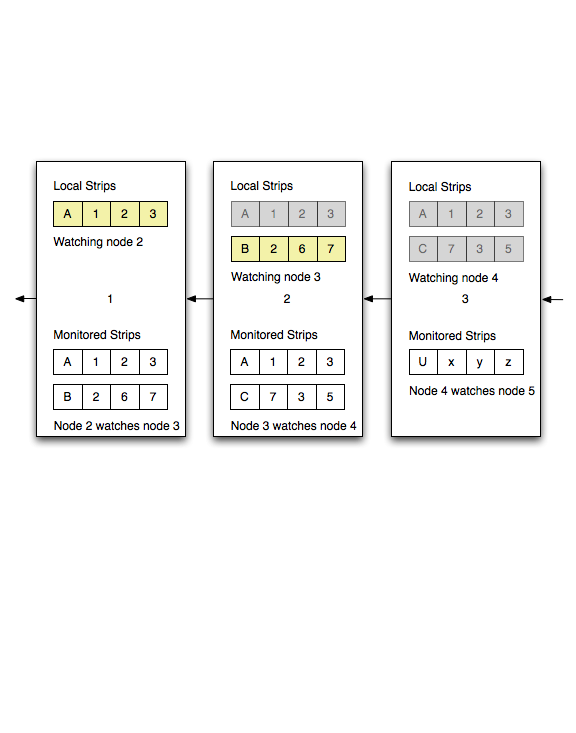
\includegraphics[width=\linewidth]{figures/strip1}
\end{figure}

Representing a component in WuKong application, each Strip contains a list of
node on which the WuObjects representing the component are hosted. As seen from
the figure~\ref{fig:strip1}, each node represented by a big white block contains
a copy of strips for components that are specified to have redundancy in fault
tolerance policy. Nodes holding a duplicated WuObject are members of the strip.
The membership of a strip is called the view. Only the WuObject hosting at the
head of the strip will be active, while the rest are backups.  As seen from
figure~\ref{fig:strip1}, node 1 has a active WuObject for component A as shown
highlighted in yellow, but duplicated WuObjects A in node 2 and 3 are inactive
in grey. In Strips, when one member failed, the next one will take over. For
instance, if a strip is constructed like this $\rightarrow 1-2-3-4-5$, when
3 failed 4 will take over the place of 3, and the new chain will look like this:
$\rightarrow 1-2-4-5$. Now if 1 failed, 2 will take over which would result in
$\rightarrow 2-4-5$, since node 2 is now at the head of the strip, its WuObject
will be active. 

Typically, there would be multiple components deployed to the network and each
node could carry multiple WuObjects, therefore many of these strips in the
network would crisscross with one and others. It is not unlikely to see a node
carrying active and inactive WuObjects at once.

\subsection{Decentralized Failure Detection}
\label{s:dfd}

%Note to self: mention single-hop, multi-hop in limitations or future work
Distributed failure detection enables high-availability in distributed systems
where partial failures is rather common.  We utilize heartbeats to detect
failures, a common technique widely used to detect failures in high-availability
distributed systems.  Heartbeats are messages sent periodically until it's
unable to send messages anymore. Each node is therefore suspected dead when
others stopped receiving messages from it after an extended period of time.
Nodes were assumed to fail by stopping and will never come back.

There are abundant literature on designing heartbeat protocols to ensure
high-availability for distributed systems. Our work employed a heartbeat
protocol arranged in such as way where each node sends a heartbeat to the
previous node and the last node sends back to the first node forming a daisy
chain as represented by the black arrows in figure~\ref{fig:strip1}.

To prevent tight coupling and redundancy in heartbeats, strips are separated
from heartbeats so the order of the strip does not affect the ordering of
heartbetas and vice versa. The heartbeat protocol is a support layer below
strips, the layers above will take advantage of the given information from the
layer below to recover the system.

\subsection{Failure Recovery}
\label{s:fr}

When a failure is detected, there are two tasks that the system would have to do
to recover from failures. First it has to make sure all members that carries
the strips in the failure nodes will have consistent view of the strips.
Second, it would need to propagate the changes to reconfigure other parts of
the system that depend on the locations of the heads of the affected strips in
order to function. The details of each task is described in the following
sections.

\subsubsection{Consistent view of strips}

\begin{figure}[h!]
\caption{A failure occurred at node 2 in the network}
\label{fig:strip3}
\centering
    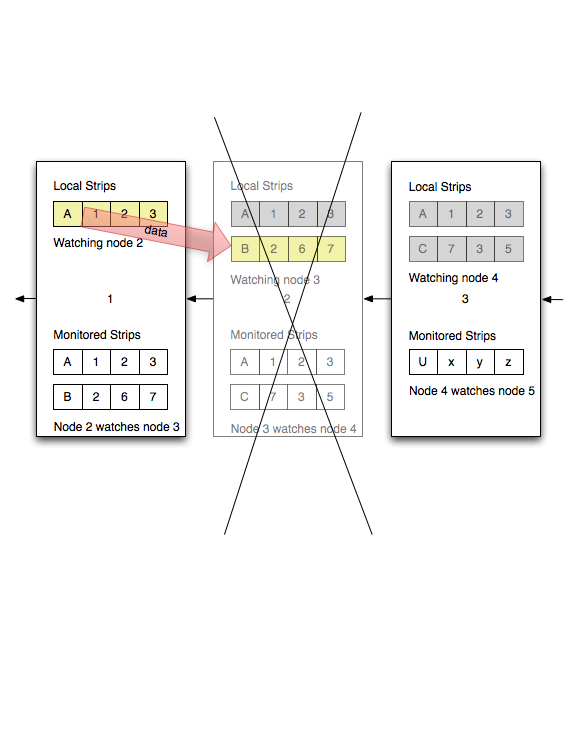
\includegraphics[width=\linewidth]{figures/strip3}
\end{figure}

Consistent view of strips is required to pick a replacement node in the event
of failure. Without consistent view, nodes will not be able to know if the
component has been replaced.
For example, in figure~\ref{fig:strip3}, when node 2 failed, node 1 will detect
this, but without algorithms to maintain consistency, node 3 would not be
certain if node 1 or 2 are still alive, thus it might take actions that could
compromise the network.

But detector might not know which strips the monitoring node is a member of, so
every node will have a copy of its monitoring node's strips view as shown in
figure~\ref{fig:strip1} below the "Monitored Strips" section where node 1 has
knowledge of the strips views of its monitoring node 2.

\begin{algorithm}
\label{alg:recovery}
\begin{pseudocode}{UpdateView}{k}
f \GETS {x}
\end{pseudocode}
\end{algorithm}

Our work proposed an algorithm attempting to recover by letting the
detector of the failure to initiate the recovery algorithms.
Since the detector will be responsible for recoverying for the failed node,
every node needs to have membership knowledge of the strips from the nodes it
is monitoring. For example, if node A is monitoring node B, A would know the
members of all strips in node B in addition to its local strips. Strips only
specifies the order of recovery, it is not correlated with the network
structure for the fault detection, in other words, a strip with A and B doesn't
mean B is monitoring A, as B could be monitored by C which depends on the
structure of heartbeat protocol layer.
In the initial algorithm, the detector node will prepare a update message to
inform all members of the strips with which the failed node is associated with.
Assuming that every node that monitors other node will have knowledge of the
strips that it contains and the members that the strips pertain. The node would
send out a marker message first to confirm the nodes which are still
functioning, and once all acknowledges have been received, it will proceed to
send the update message to update their local knowledge of the strips to reach
a consensus. The ordering of the messages wouldn't matter since the end state
of any failure sequence for any strip would be the same. For example, given
a strip of three members $\rightarrow 1-2-3$, if the updated failure sequence
is given in any permutation by $[1, 2]$ or $[2, 1]$, the end results would be
the same $\rightarrow 3$ since the remaining members from those two failure
sequence is the same and the relative order of the members would stay the same.
\begin{comment}
Let's assume there is a pair of failure patterns with the same members but
different orders that would do update operations on the same strip but would
leave the strip in different results. If that's true, then by building back the
strips from the result in the order of update operations would result in
a different starting state, that implies the strips have different members or
member orders to start with, a contradiction.
\end{comment}
Therefore there is no need for extra communication overhead to maintain
ordering to gaurantee level of consistency between members since they will all
come to the same conclusion given each receiver receive the same messages. The
overhead are messages required to update each member's internal membership
information.

\subsubsection{Reconfiguration}
\label{s:reconfig}

\begin{figure}[h!]
\caption{A reconfiguration of a Network}
\label{fig:reconfig-network}
\centering
    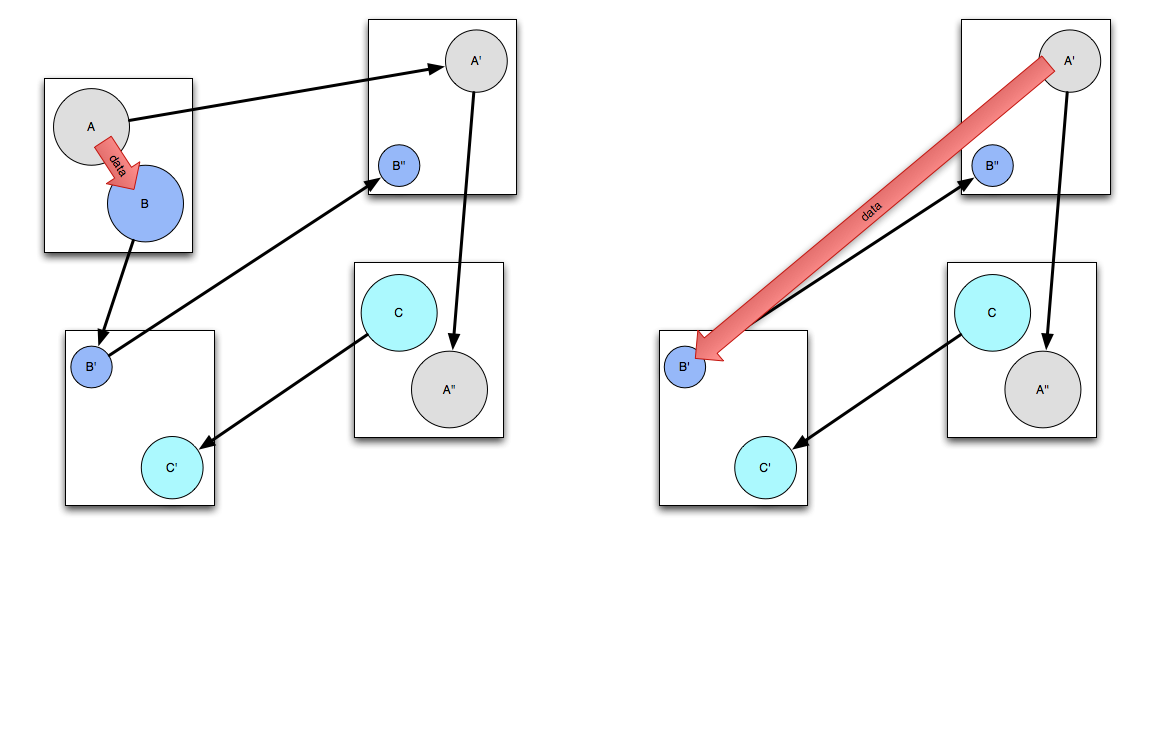
\includegraphics[width=\linewidth]{figures/reconfig-network}
\end{figure}

Even though consensus of the new configuration for each affected strip has been
reached, some nodes with component that acts as a client to another component
for data or the reverse would also have to have consensus on the updated
primary holder of each affected component. And the node that is monitoring the
node monitored by the dead node would also need to update on its knowledge of
its monitored node in order to recover the next possible failure.

RASCO will initiate a reconfiguration service to reconfigure the network to adapt
to the new strip configurations. Reconfiguration service is implemented by
a distributed algorithm which is inititated by the detected nodes. First the
initiator node would have to identify the components that are reading/writing
data with the components carried by the dead host. This would be done by
requesting the link information between components at the higher level provided
by the application. Then each member of the strips of the connected components
would be updated with the information about the change in the host of the
failed components with a \emph{reconfig} message containing the change in the
location of the specific WuObjects. Right after receiving the \emph{reconfig}
message, if the connected nodes whose WuObjects are pushing data to the
WuObjects on the failed nodes, they will force to initiate a data push to
update and bring the recovered nodes up to date, and vice versa, so the nodes
whose WuObjects are receiving data from the failed nodes will initiate a data
pull after receiving the \emph{reconfig} message.

As shown in figure~\ref{fig:reconfig-network}, the network on the right has
a node failed that bring both current heads of strips A, and B down. As shown
on the right, after recovery, the nodes that have the active WuObjects
connecting to each new heads in both strips A and B both will be updated on the
current location of the heads of both strips. Because the bottom left node
contains the new head of strip B and is connected to strip A, therefore it will
be updated on the location of the new head of strip B, and vice versa.

Reconfiguration service has message complexity of $O(m)$ where m is the
number of strips where its components are linked to the failed components.


\subsection{System Implementation}

